\documentclass{scrartcl}

\usepackage{amssymb}
\usepackage{amsmath}
\usepackage{tikz}
\usetikzlibrary{arrows, arrows.meta}
\frenchspacing

%Serres - The Birth of Physics, pp. 19 & 76

\begin{document}
	
	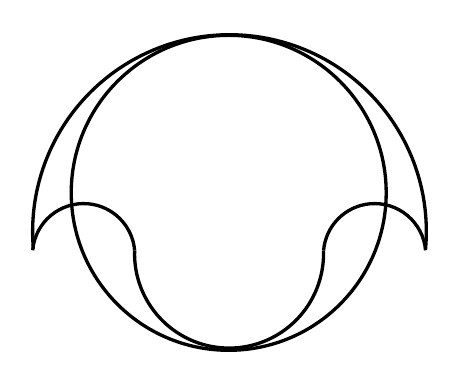
\begin{tikzpicture}		%σαλινον
	\draw[very thick] (0,0) circle (2cm);					%center circle
	\draw[very thick] (2.5,-0.71) arc (-5:185:2.5cm);		%upper arc
	\draw[very thick] (-2.49,-0.73) arc (175:5:0.65cm);		%left arc
	\draw[very thick] (2.5,-0.73) arc (5:175:0.65cm);		%right arc
	\draw[very thick] (-1.195,-0.73) arc (178:362:1.2cm);	%bottom arc
	\end{tikzpicture}
	
	\vspace{2.5cm}
	
	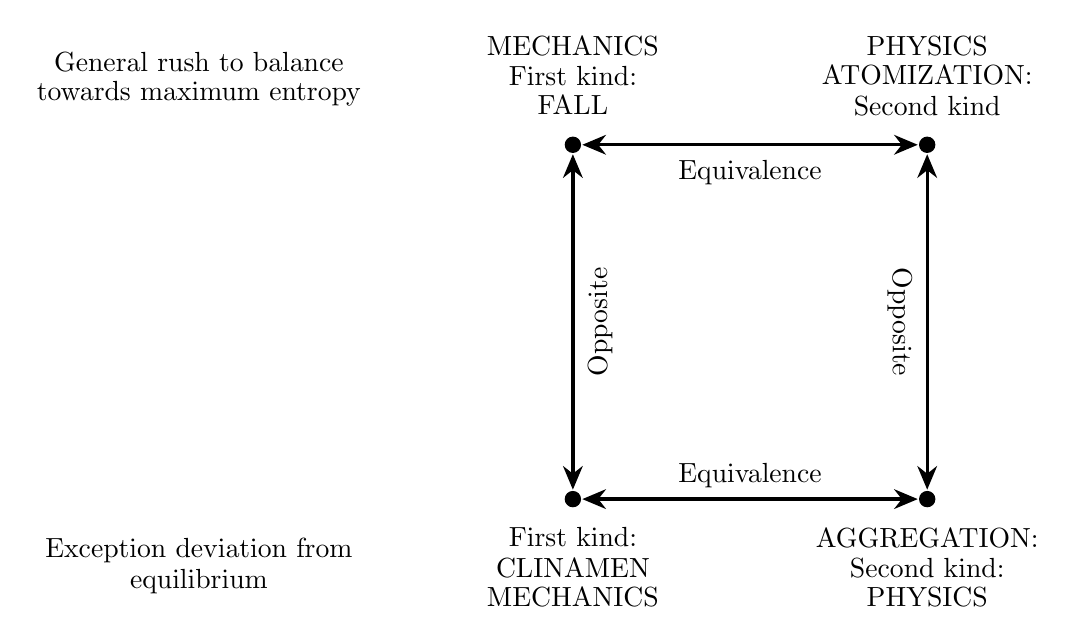
\begin{tikzpicture}
	%outside labels
	\node at (-7,3.3) {General rush to balance};
	\node at (-7,2.9) {towards maximum entropy};
	%
	\node at (-2.25,3.5)  {MECHANICS};
	\node at (-2.25,3.12) {First kind:};
	\node at (-2.25,2.75) {FALL};
	%
	\node at (2.25,3.5)  {PHYSICS};
	\node at (2.25,3.13) {ATOMIZATION:};
	\node at (2.25,2.75) {Second kind};
	%
	\node at (-2.25,-2.73) {First kind:};
	\node at (-2.25,-3.13) {CLINAMEN};
	\node at (-2.25,-3.5)  {MECHANICS};
	%
	\node at (2.25,-2.75) {AGGREGATION:};
	\node at (2.25,-3.12) {Second kind:};
	\node at (2.25,-3.5)  {PHYSICS};
	%
	\node at (-7,-2.9) {Exception deviation from};
	\node at (-7,-3.3) {equilibrium};
	
	%circles
	\node[circle,draw=black,fill=black,inner sep=0pt,minimum size=5.5pt] at (2.25,2.25)  {};
	\node[circle,draw=black,fill=black,inner sep=0pt,minimum size=5.5pt] at (-2.25,2.25) {};
	\node[circle,draw=black,fill=black,inner sep=0pt,minimum size=5.5pt] at (2.25,-2.25) {};
	\node[circle,draw=black,fill=black,inner sep=0pt,minimum size=5.5pt] at (-2.25,-2.25){};
	
	%arrows - if increasing arrowhead size, must do one arrow for each direction
	\draw [-{Stealth[length=3mm,width=2.5mm]},very thick] (-2,2.25)--(2.13,2.25);
	\draw [-{Stealth[length=3mm,width=2.5mm]},very thick] (2,2.25)--(-2.13,2.25);
	%
	\draw [-{Stealth[length=3mm,width=2.5mm]},very thick] (2.25,-2)--(2.25,2.13);
	\draw [-{Stealth[length=3mm,width=2.5mm]},very thick] (2.25,2)--(2.25,-2.13);
	%
	\draw [-{Stealth[length=3mm,width=2.5mm]},very thick] (-2.25,-2)--(-2.25,2.13);
	\draw [-{Stealth[length=3mm,width=2.5mm]},very thick] (-2.25,2)--(-2.25,-2.13);
	%
	\draw [-{Stealth[length=3mm,width=2.5mm]},very thick] (-2,-2.25)--(2.13,-2.25);
	\draw [-{Stealth[length=3mm,width=2.5mm]},very thick] (2,-2.25)--(-2.13,-2.25);
	
	%inside labels
	\node at (0,1.9)  {Equivalence};
	\node at (0,-1.95){Equivalence};
	\node at (-1.9,0) {\rotatebox{90}{Opposite}};
	\node at (1.9,0)  {\rotatebox{270}{Opposite}};
	\end{tikzpicture}
	
	\vspace{0.25cm}
	
	\begin{quote}
		{\small The universal law of the rush to equilibrium is double. If it is the fall of heavy bodies, it is mechanics, if it is automation, it is physics. The fall is the mechanical equivalent of atomisation, and it is more simple. It says, in pure movement, what dissemination says in matter. Now, if something exists, this is because aggregation takes place, physically speaking, by and in matter. There is an exception to the general rule of irreversible atomisation. Hence its mechanical equivalent, simpler in pure movement: the \textit{clinamen}, as a local deviation from equilibrium.}
	\end{quote}
	
\end{document}